\documentclass[portrait, a0paper, margin=.5cm]{baposter}

\usepackage{poster_style}

\begin{document}
    \begin{poster}%
    {
        grid=false,
        eyecatcher=true,
        bgColorOne=white,
        bgColorTwo=white,
        borderColor=IGNGrey,
        headerColorOne=IGNGrey,
        headerColorTwo=IGNGrey,
        headerFontColor=white,
        boxColorOne=white,
        boxColorTwo=white,
        colspacing=.5em,
        columns=6,
        textborder=rounded,
        headerborder=closed,
        headerheight=0.12\textheight,
        headershape=rounded,
        textfont={\color{IGNDarkGrey}},
        boxshade=plain,
        background=none,
        linewidth=1pt
    }
    {}
    {
        \color{IGNDarkGrey}
        The necessary yet complex evaluation of 3D city\\models: a semantic approach
    }
    {
        \vspace{.5cm}
        \color{IGNDarkGrey}
        \begin{tabular}{c c}
            \small Oussama Ennafii, Clément Mallet, Arnaud Le Bris & \small Florent Lafarge\\
            \small Univ. Paris Est, IGN-ENSG, LaSTIG, Saint-Mandé, France & \small Inria, TITANE, Sophia Antipolis, France\\
            \small firstname.secondname@ign.fr & \small florent.lafarge@inria.fr
        \end{tabular}
    }
    {
        \begin{tabular}{c}
            
\includegraphics[width=2.2cm]{images/logos/ign_logo}\\~\\
            
\includegraphics[width=2.2cm]{images/logos/paris_est_logo}
        \end{tabular}
    }

        \TransitionBox{motivation}{}{{\large \sc Motivation:} automatically evaluating building models.}

        \StandardBox{context}{column=0, span=2, row=.03}{Context}{
            \begin{itemize}[label=, leftmargin=*]
                \item A wide application range~\cite{Biljecki2015} for urban models;
                \item Automatic urban modeling: active research area~\cite{Musialski2012}, but {\color{red}not yet fully operational};
                \item Approximately, \SI{2}{\hour \per\square \kilo\meter} per expert to assess 3D model quality.
            \end{itemize}
        }
        \StandardBox{potential}{column=2, span=2, aligned=context, bottomaligned=context}{Potential use}{
            \begin{itemize}[label=--, leftmargin=*]
                \item Change detection;
                \item Urban models correction;
                \item Urban reconstruction method evaluation;
                \item Crowd reconstruction quality assessment.
            \end{itemize}
        }
        \StandardBox{state_art}{column=4, span=2, aligned=context, bottomaligned=context}{State of the art classification}{
            According to the output:
            \begin{itemize}[label=--, leftmargin=1em]
                \item {\color{IGNGreen} geometric fidelity metrics} usually comparing to {\color{orange} higher precision} reference models~\cite{vogtle2003quality, Henricsson1997}.
                \item {\color{IGNGreen} semantic errors} relying on remote sensing data (LiDAR, DSM, Orthoimage)~\cite{Akca2010, OudeElberink2010, boudet2006supervised, Michelin2013}.
            \end{itemize}
        }
        \StandardBox{graphical_abstract}{column=0, span=6, below=context}{Proposed strategy}{
            \begin{multicols}{2}
                \includestandalone[mode=buildnew, width=.5\textwidth]{graphical_abstract}
                \begin{itemize}[label=--, leftmargin=1.5em]
                    \item A new \textcolor{IGNGreen}{taxonomy of errors} hierarchical and independent from input models;
                    \item A \textcolor{IGNGreen}{supervised classification} formulation of the problem;
                    \item A multimodal (intrinsic and extrinsic) \textcolor{IGNGreen}{baseline of features}.
                \end{itemize}
            \end{multicols}
        }
        
        \TransitionBox{formul}{below=graphical_abstract}{{\large \sc Problem formulation:} using intrinsic and possibly extrinsic features to predict model quality.}

        \StandardBox{taxonomy}{column=0, span=3, row=.34}{Error taxonomy: overhead modeling case}{
            \includestandalone[mode=buildnew, width=\textwidth]{taxonomy_tree}
        }

        \StandardBox{samples}{column=3, span=3, aligned=taxonomy}{Errors samples}{
            \begin{multicols}{4}
                \begin{center}
                    \fbox{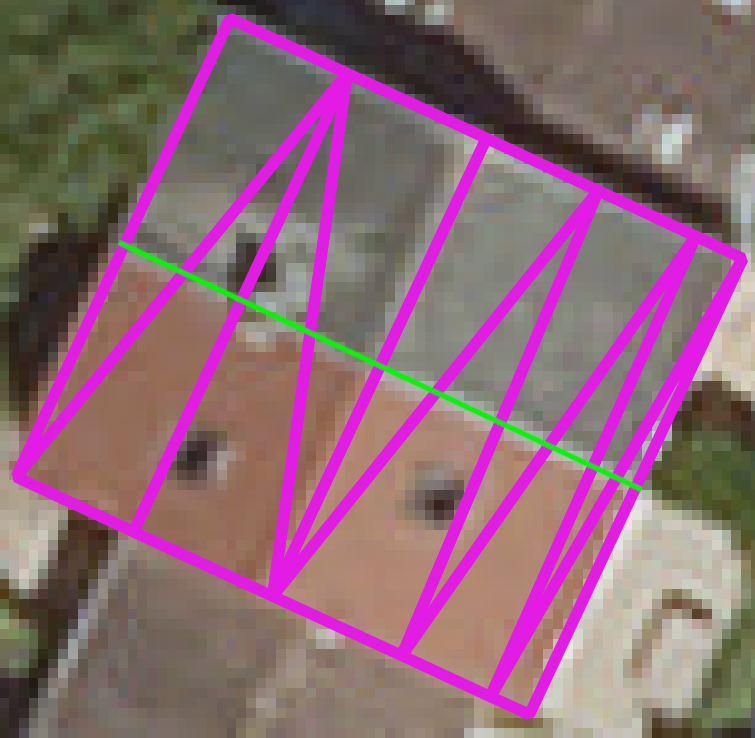
\includegraphics[height=1.75cm]{images/errors/building/under_segmentation}}
                    \captionof*{figure}{\scriptsize \texttt{BUS}}
                \end{center}
                \begin{center}
                    \fbox{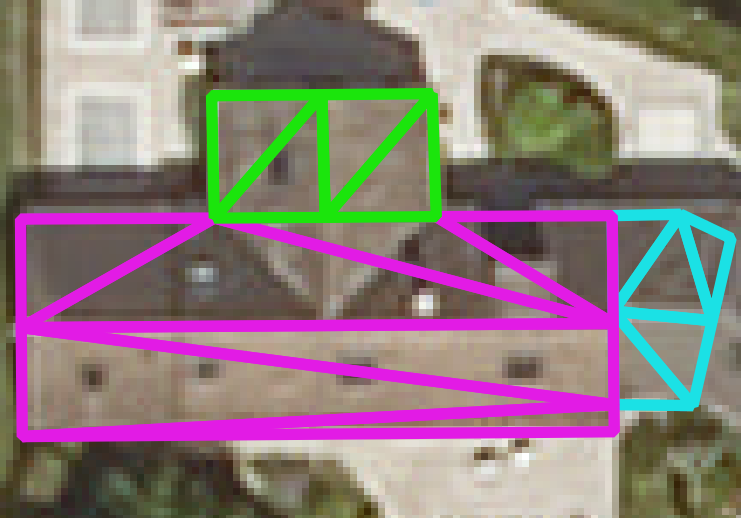
\includegraphics[height=1.75cm]{images/errors/building/over_segmentation}}
                    \captionof*{figure}{\scriptsize \texttt{BOS}}
                \end{center}
                \begin{center}
                    \fbox{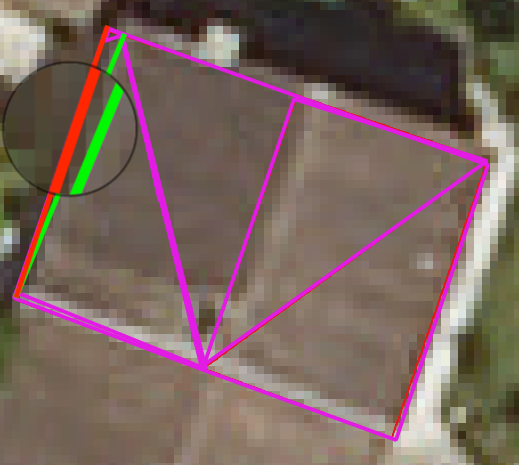
\includegraphics[height=1.75cm]{images/errors/building/border}}
                    \captionof*{figure}{\scriptsize \texttt{BIB}}
                \end{center}
                \begin{center}
                    \fbox{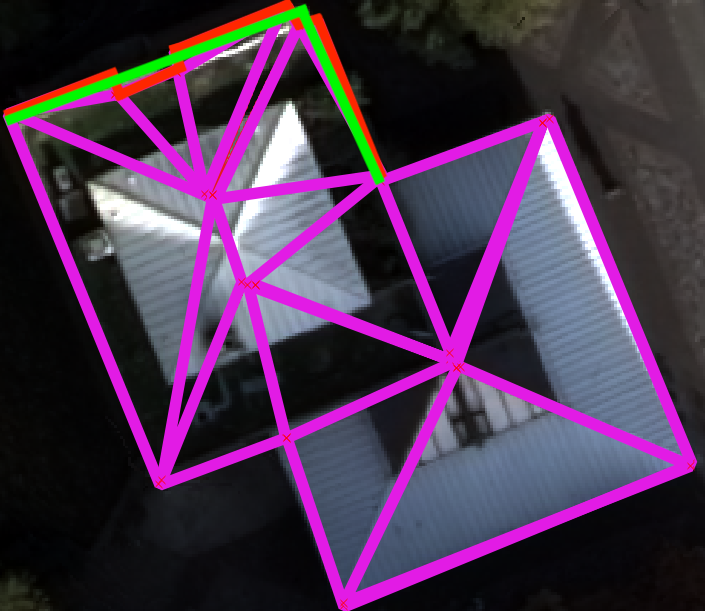
\includegraphics[height=1.75cm]{images/errors/building/topology}}
                    \captionof*{figure}{\scriptsize \texttt{BIT}}
                \end{center}
            \end{multicols}
            \begin{multicols}{5}
                \begin{center}
                    \fbox{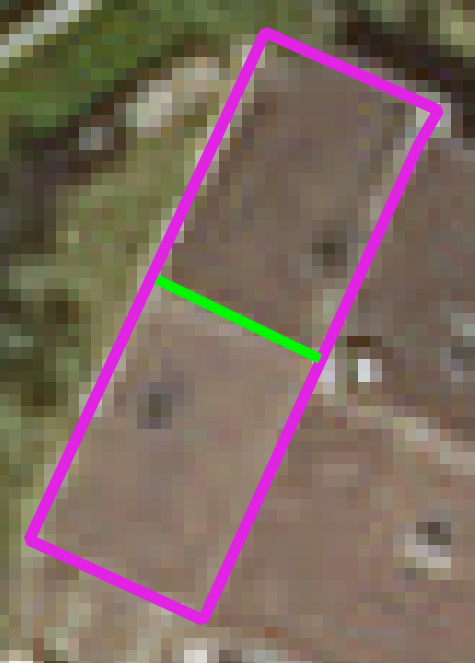
\includegraphics[height=1.45cm]{images/errors/facet/under_segmentation}}
                    \captionof*{figure}{\scriptsize \texttt{FUS}}
                \end{center}
                \begin{center}
                    \fbox{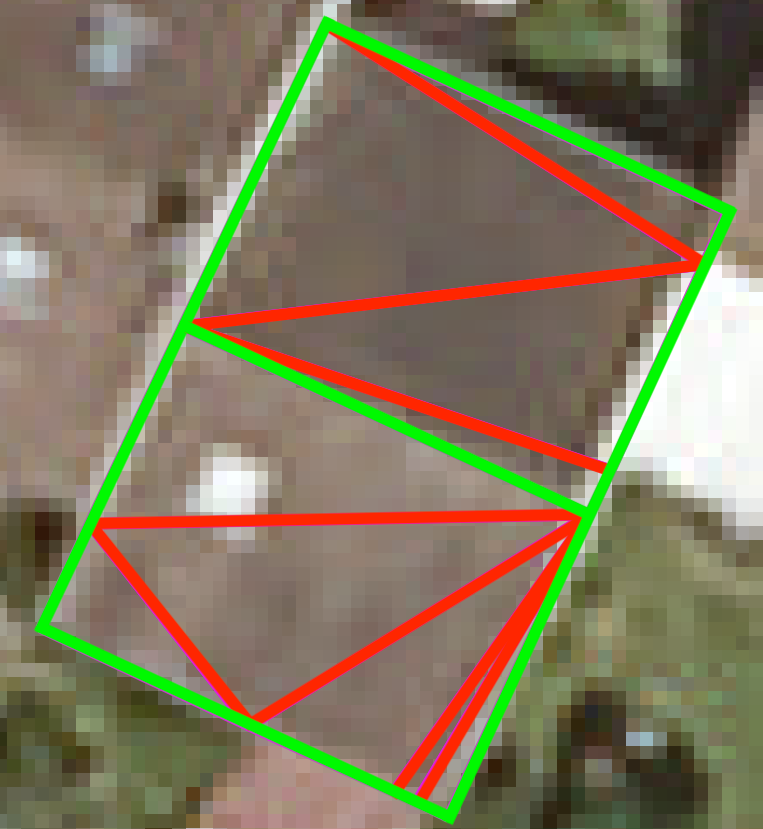
\includegraphics[height=1.45cm]{images/errors/facet/over_segmentation}}
                    \captionof*{figure}{\scriptsize \texttt{FOS}}
                \end{center}
                \begin{center}
                    \fbox{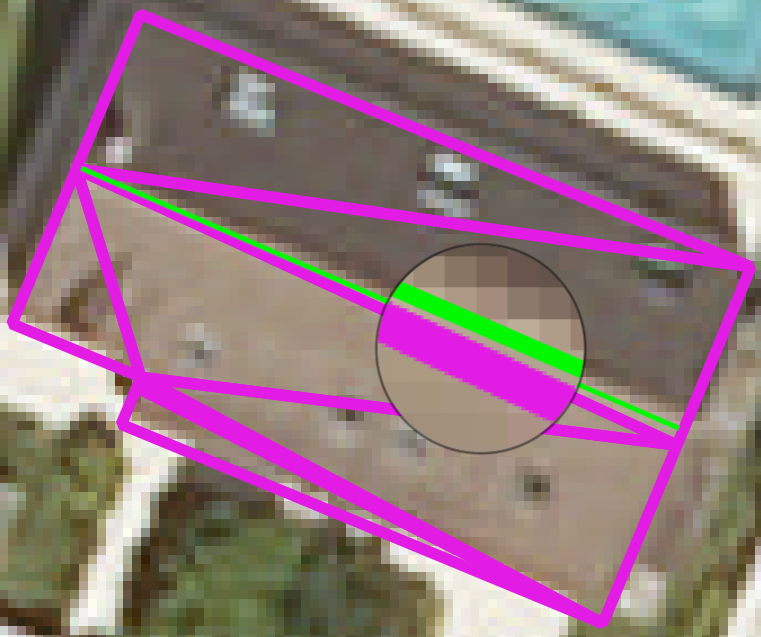
\includegraphics[height=1.45cm]{images/errors/facet/border}}
                    \captionof*{figure}{\scriptsize \texttt{FIB}}
                \end{center}
                \begin{center}
                    \fbox{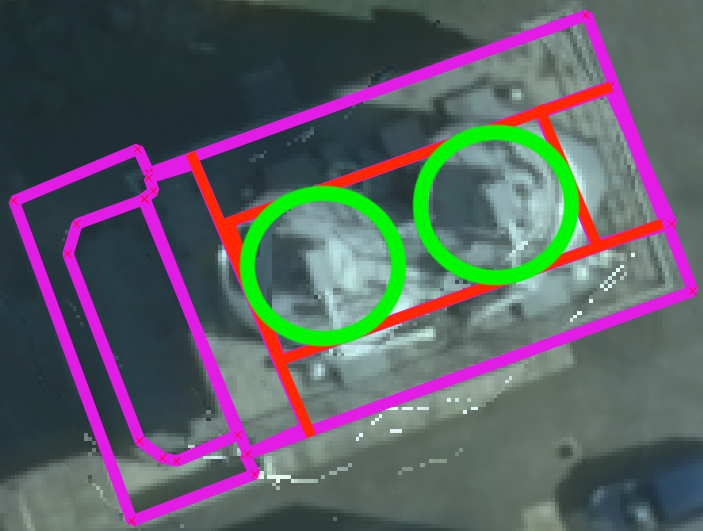
\includegraphics[height=1.45cm]{images/errors/facet/topology}}
                    \captionof*{figure}{\scriptsize \texttt{FIT}}
                \end{center}
                \begin{center}
                    \fbox{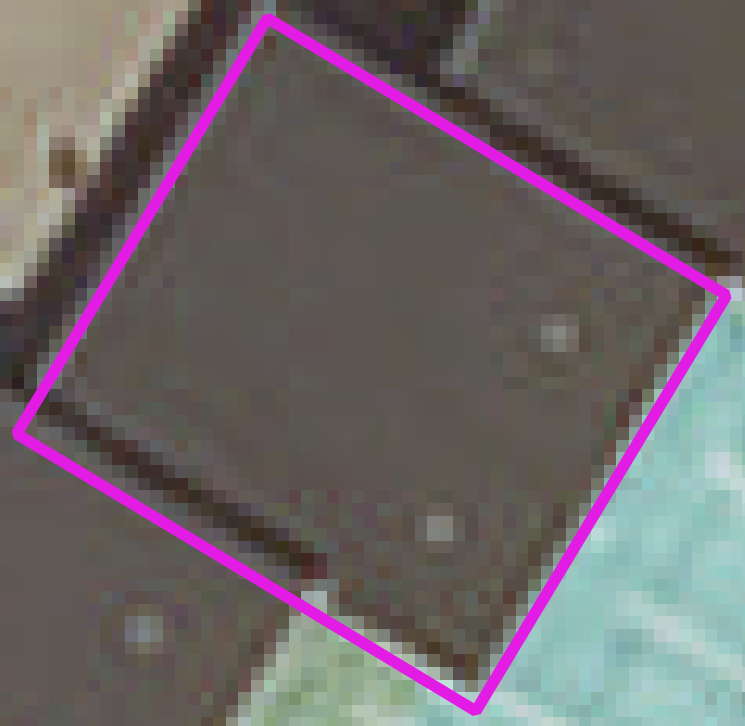
\includegraphics[height=1.45cm]{images/errors/facet/geometry}}
                    \captionof*{figure}{\scriptsize \texttt{FIG}}
                \end{center}
            \end{multicols}
        }
        
         \StandardBox{dataset}{column=0, span=3, below=taxonomy}{Datasets}{
            \begin{center}
        		\scriptsize
                \begin{tabular}{c c c c}
                    \toprule
                    & \textbf{Elancourt} & \textbf{Nantes} & \textbf{Paris-13} \\
                    \midrule
                    \# samples & 2009 & 748 & 478 \\
                    DSM res. & \SI{6}{\cm} & \SI{10}{\cm} & \SI{10}{\cm} \\
                    Img. res. & \SI{6}{\cm} & \SI{10}{\cm} & \SI{10}{\cm} \\
                    Typology & bi-level + flat roof & dense city center & Haussmann style + high towers \\
                    \bottomrule
                \end{tabular}
        	\end{center}
         }
        
        \StandardBox{ablation}{column=0, span=3, below=dataset}{Ablation study: Elancourt case (10-fold cross val.)}{
            \begin{center}
                \scriptsize
                \begin{tabular}{|x{.7cm} | x{.8cm} x{.8cm} | x{.8cm} x{.8cm} | x{.8cm} x{.8cm} | x{.8cm} x{.8cm}|}
        			\hline
                    &\multicolumn{2}{x{1.6cm}|}{\textbf{Geom.}} & \multicolumn{2}{x{1.6cm}|}{\textbf{Geom. $\cup$ Hei.}} & \multicolumn{2}{x{1.6cm}|}{\textbf{Geom. $\cup$ Im.}} & \multicolumn{2}{|x{1.6cm}|}{\textbf{All}}\\
                    \cline{2-9}
                    &\textbf{Rec.} & \textbf{Prec.} & \textbf{Rec.} & \textbf{Prec.} & \textbf{Rec.} & \textbf{Prec.} & \textbf{Rec.} & \textbf{Prec.}\\
                    \hline
                    \textit{\texttt{BOS}} & \textbf{93.96} & 76.15 & 91.43 & \textbf{77.76} & 91.51 & 76.08 & 90.83 & 76.14 \\
                    \hline
                    \textit{\texttt{BUS}} & 32.98 & \textbf{76.47} & \textbf{41.86} & 75.57 & 40.38 & 71.00 & 39.32 & 71.81 \\
                    \hline
                    \textit{\texttt{BIB}} & 12.32 & 67.57 & 12.81 & \textbf{68.42} & 16.26 & 67.35 & \textbf{16.75} & 68.0 \\
                    \hline
                    \textit{\texttt{BIT}} & \textbf{25.25} & 92.59 & 20.20 & 90.91 & 20.20 & \textbf{95.24} & 11.11 & 91.67 \\
                    \hline
                    \hline
                    \textit{\texttt{FOS}} & 98.91 & 99.07 & 98.91 & \textbf{99.30} & \textbf{98.99} & 98.84 & 98.91 & 98.84 \\
                    \hline
                    \textit{\texttt{FUS}} & \textbf{1.90} & 54.55 & 0.63 & \textbf{66.67} & 1.61 & 50 & 1.27 & \textbf{66.67} \\
                    \hline
                    \textit{\texttt{FIB}} & \textbf{9.17} & 87.5 & 0 & --- & 8.30 & 82.61 & 7.42 & \textbf{100} \\
                    \hline
                    \textit{\texttt{FIT}} & \textbf{6.67} & \textbf{100} & 8.73 & 95.24 & 3.33 & \textbf{100} & 3.33 & \textbf{100} \\
                    \hline
                    \textit{\texttt{FIG}} & \textbf{80.54} & 73.14 & 80.45 & \textbf{72.62} & 78.69 & 72.12 & 79.02 & 71.82 \\
                    \hline
        		\end{tabular}
            \end{center}
        }
        
        \StandardBox{scalability}{column=3, span=3, below=samples, bottomaligned=ablation}{Scalability study}{
            \begin{center}
                \smaller
                    The color indicates the change magnitude: \textcolor{Moins4}{$\blacksquare$}: $[-45,-35\%[$-- \textcolor{Moins3}{$\blacksquare$}: $[-35,-25\%[$ -- \textcolor{Moins2}{$\blacksquare$}: $[-25,15\%[$-- \textcolor{Moins1}{$\blacksquare$}: $[-15, 5\%[$ -- $\square$: $[-5,5\%[$-- \textcolor{Plus1}{$\blacksquare$}: $[5,15\%[$ -- \textcolor{Plus2}{$\blacksquare$}: $[15,25\%]$ -- $\blacksquare$: cannot be computed.\\

                    \begin{tabular}{c c| x{.4cm} x{.4cm} x{.4cm} x{.4cm} |x{.4cm} x{.4cm} x{.4cm} x{.4cm} x{.4cm}}
                        \hline
                        &&\texttt{BOS}  & \texttt{BUS} &\texttt{BIB} &\texttt{BIT} &\texttt{FOS}  & \texttt{FUS} &\texttt{FIB} &\texttt{FIT} &\texttt{FIG} \\
                        \hline
                        \multirow{6}{*}{\rotatebox{90}{Transferability}}&El. $\rightarrow$ Na. &\cellcolor{Moins1} & \cellcolor{Moins2}&\cellcolor{Moins1}& \cellcolor{Moins2}& \cellcolor{Zero}& \cellcolor{Zero}&\cellcolor{Plus2} Im. & \cellcolor{Moins1}&\cellcolor{Zero}\\
                        &El. $\rightarrow$ P-13  & \cellcolor{Moins1}& \cellcolor{Moins2}& \cellcolor{Zero}& \cellcolor{Moins2}& \cellcolor{Zero}& \cellcolor{Plus1}Im.& \cellcolor{Plus1}Im.& \cellcolor{Moins1}&\cellcolor{Zero}\\
                        &Na. $\rightarrow$ P-13  & \cellcolor{Moins1}& \cellcolor{Moins2}& \cellcolor{black} & \cellcolor{Plus2}& \cellcolor{Zero}& \cellcolor{Plus1}& \cellcolor{Plus1}& \cellcolor{black} &\cellcolor{Zero}\\
                        &Na. $\rightarrow$ El.  &\cellcolor{Plus1} & \cellcolor{Moins1}& \cellcolor{Moins1}&\cellcolor{Plus1}All & \cellcolor{Zero}& \cellcolor{Moins2}&\cellcolor{Moins1}Im. &\cellcolor{Plus1}Im. &\cellcolor{Zero}\\
                        &P-13 $\rightarrow$ Na.  &\cellcolor{Moins2} & \cellcolor{Moins1}& \cellcolor{black} & \cellcolor{Plus1}&\cellcolor{Zero} & \cellcolor{Moins3}& \cellcolor{Zero}& \cellcolor{black} & \cellcolor{Moins1} Hei.\\
                        &P-13 $\rightarrow$ El. &\cellcolor{Zero} &\cellcolor{Moins1} & \cellcolor{Plus1}Im. & \cellcolor{Zero}& \cellcolor{Zero}& \cellcolor{Moins4}& \cellcolor{Moins2}Im. & \cellcolor{black} & \cellcolor{Zero}\\
                        \hline
                        \multirow{3}{*}{\rotatebox{90}{General.}  }&El.   & \cellcolor{Moins2}& \cellcolor{Moins2}Im.& \cellcolor{Moins2}&\cellcolor{Moins2} &\cellcolor{Zero} &\cellcolor{Plus1}Im. &\cellcolor{Plus2}Im. &\cellcolor{Moins1}Geom. & \cellcolor{Moins1} Hei\\
                        &Na.   & \cellcolor{Zero}All& \cellcolor{Moins2}Im.&\cellcolor{Moins1}Im. &\cellcolor{Plus2} &\cellcolor{Zero} & \cellcolor{Zero}& \cellcolor{Moins2}Im.& \cellcolor{black} &\cellcolor{Zero}\\
                        &P-13   &\cellcolor{Moins2}All &\cellcolor{Moins2} & \cellcolor{black} &\cellcolor{Plus1}Hei. &\cellcolor{Zero} &\cellcolor{Moins4} &\cellcolor{Moins2}Im. & &\cellcolor{Moins1}\\
                        \hline
                    \end{tabular}
                \end{center}
        }
        \StandardBox{conclusion}{column=0, span=3, below=ablation}{Conclusion}{
            \begin{itemize}[label=--, leftmargin=1em]
                \item Flexible, robust and hierarchical taxonomy;
                \item Fast, lightweight and modular pipeline for model evaluation;
                \item Baseline for geometric, image-based and height-based features.
            \end{itemize}
        }
        \StandardBox{perspectives}{column=3, span=3, aligned=conclusion, bottomaligned=conclusion}{Perspectives}{
            \begin{itemize}[label=--, leftmargin=1em]
                \item Simulating errors $\longrightarrow$ more training samples;
                \item Structurally aware features: graph kernels, scattering transforms \dots;
                \item A 3D city modeling benchmark proposal.
            \end{itemize}
        }

        \ReferencesBox{references}{column=0, span=5, below=perspectives}{\bf{References}}{
            \setlength{\columnseprule}{0.1pt}
            \begin{multicols}{3}
                \renewcommand{\section}[2]{}
                \bibliographystyle{abbrv}
                \tiny \bibliography{short_references}
            \end{multicols}
        }

        \InvisibleBox{qr}{column=5, span=1, below=perspectives}{}{
            \begin{center}
                
\includegraphics[width=.9\textwidth]{images/qr}
            \end{center}
        }

        \InvisibleBox{event}{column=2, span=2, row=.985}{}{
            \begin{tikzpicture}
                \node[rectangle, minimum width=\textwidth]{
                    \footnotesize{JURSE 2019}
                };
            \end{tikzpicture}
        }
    \end{poster}
\end{document}
